\section{Convolutional and Transformer Models}
\label{sec:cnn_transformer}

Both models read the same window as the recurrent networks of Section~\ref{sec:recurrent}: $X=(x_1,\dots,x_T)$ with $T=30$ cycles and $x_t\in\mathbb{R}^{14}$, standardised with training-engine statistics.  Each model maps $X$ to a pooled vector $z\in\mathbb{R}^{d}$ and predicts $\hat y=w^\top z+b$, trained with the same loss, optimiser (AdamW~\cite{loshchilov_2019_adamw}), early stopping and selection rule as the recurrent models.

\subsection{One-dimensional CNN}
A convolutional layer with kernel size $k$ and dilation $\delta$ computes, for output channel $c'$ and position $t$,
\begin{equation}
h^{(c')}_t=\mathrm{ReLU}\!\Big(b_{c'}+\sum_{c=1}^{C_{\mathrm{in}}}\sum_{j=-(k-1)/2}^{(k-1)/2} w_{c',c,j}\,x^{(c)}_{t+\delta j}\Big),
\end{equation}
where $w$ are the learned filters, $b$ the biases and $C_{\mathrm{in}}$ the number of input channels, with zero padding at the window ends.  Stacking $L$ layers with dilations $\delta_1,\dots,\delta_L$ gives every position a receptive field of
\begin{equation}
R=1+(k-1)\sum_{l=1}^{L}\delta_l
\end{equation}
cycles.  Global average pooling $z=\frac{1}{T}\sum_{t}h_t$ then summarises the window.  Symmetric padding is safe because a window already ends at the current cycle, so every position lies in the past.  The starter model ($L=2$, $k=5$, $\delta=1$) had $R=9$.  We changed one factor at a time: normalisation (batch~\cite{ioffe_2015_batchnorm} or layer~\cite{ba_2016_layernorm}), residual connections $h\leftarrow h+F(h)$~\cite{he_2016_resnet}, pooling (average, maximum, last step), dilation, depth and kernel size.  Convolutional regression networks have been used for RUL before~\cite{babu_2016_dcnn,li_2018_dcnn}, and dilated convolutions are the basis of temporal convolutional networks~\cite{bai_2018_tcn}.

\subsection{Transformer encoder}
The Transformer replaces recurrence by self-attention~\cite{vaswani_2017_transformer}.  A linear layer projects each $x_t$ to $d_{\mathrm{model}}=32$ and a positional encoding is added, because attention alone ignores order:
\begin{align}
\mathrm{PE}(t,2i)&=\sin\!\big(t/10000^{2i/d_{\mathrm{model}}}\big),\\
\mathrm{PE}(t,2i{+}1)&=\cos\!\big(t/10000^{2i/d_{\mathrm{model}}}\big).
\end{align}
With $Q$, $K$, $V$ the query, key and value projections of the sequence and $d_k$ the key size, one head computes
\begin{equation}
\mathrm{Attention}(Q,K,V)=\mathrm{softmax}\!\Big(\frac{QK^\top}{\sqrt{d_k}}\Big)V,
\end{equation}
where the division by $\sqrt{d_k}$ keeps the dot products from growing with $d_k$ and saturating the softmax.  Multi-head attention concatenates $h$ heads (here 4) and projects them with $W^O$.  Each of the $N$ blocks is a pre-norm residual block,
\begin{equation}
X'=X+\mathrm{MHA}(\mathrm{LN}(X)),\qquad X''=X'+\mathrm{FFN}(\mathrm{LN}(X')),
\end{equation}
with layer normalisation $\mathrm{LN}(u)=\gamma\odot(u-\mu)/\sqrt{\sigma^2+\epsilon}+\beta$ over the feature dimension and a feed-forward network $\mathrm{FFN}(u)=W_2\max(0,W_1u+b_1)+b_2$ of width $2d_{\mathrm{model}}$.  Mean pooling over time gives $z$.  A block has about $4d_{\mathrm{model}}^2$ attention weights and $2d_{\mathrm{model}}d_{\mathrm{ff}}$ feed-forward weights, and the attention scores cost $O(T^2d_{\mathrm{model}})$: 900 score entries per head and layer at $T=30$ and 2\,500 at $T=50$.

\subsection{Results}
Figure~\ref{fig:cnn_sweeps} shows the effect of each factor on the validation-engine window MAE.  The CNN gained most from a wider receptive field: dilation 2 and 4 ($R=17$ and $33$) lowered the window MAE from 31.36 to 29.77 and 28.86 cycles, whereas deeper stacks (3 and 4 layers) and a smaller kernel raised it, the deeper ones through overfitting (training MAE 11.9 and 10.7 against 22.0).  Layer normalisation helped (29.72) but fitted the training engines much more closely (training MAE 6.6), and a combined run of the helpful changes (29.27) was worse than dilation 4 alone, so the selection rule chose the CNN with dilation 4.  The Transformer was insensitive to most factors; three layers (27.07 against 27.82) was the selected change, and a model with 795\,393 parameters reached a training MAE of 6.5 but the same window MAE (27.76), which shows overfitting on 80 engines.

Table~\ref{tab:cnn_tr} compares the models on the 100 fixed validation points.  The CNN reached an MAE of $24.38\pm0.14$ and the Transformer $22.80\pm2.28$ cycles (mean and standard deviation over three seeds).  Both are below the Random Forest of Phase 1 (25.03), but the margins are small relative to the seed spread of the Transformer and to the sampling noise of 100 points from 20 engines.  Neither model beats the LSTM ($20.14\pm1.46$), and the Transformer is tied with the GRU.  The recurrent models are also cheaper, because the CNN and Transformer need 2.1 and 3.8 seconds per epoch against 0.67 and 1.15 for the LSTM and GRU.  No model removes the high-RUL bias: for true RUL above 200 (five points) the mean error is $-117.5$ (CNN) and $-111.9$ cycles (Transformer).  First-layer attention is spread over the window rather than focused on the latest cycles (Fig.~\ref{fig:attention}); it shows where one layer looks and does not explain a prediction.

% Source: results/phase2/summary_cnn_transformer.csv, summary_rnn.csv, model_cost.csv, results/phase1/final_results.csv
\begin{table}[t]
\centering
\caption{Validation results on the 100 fixed points (cycles). MAE and RMSE are mean $\pm$ standard deviation over seeds 42--44 (single run for Random Forest); early and late MAE are for the seed-42 model. Cost is measured on one CPU thread.}
\label{tab:cnn_tr}
\footnotesize
\resizebox{\columnwidth}{!}{%
\begin{tabular}{lccccrr}
\toprule
Model & MAE & RMSE & Early & Late & Params & s/epoch\\
\midrule
Random Forest & 25.03 & 40.17 & 49.33 & 18.17 & -- & --\\
LSTM & $20.14\pm1.46$ & $33.18\pm2.46$ & 43.73 & 12.55 & 20\,545 & 0.67\\
GRU & $22.98\pm0.49$ & $36.61\pm0.90$ & 43.34 & 17.49 & 40\,385 & 1.15\\
CNN & $24.38\pm0.14$ & $36.86\pm0.17$ & 41.33 & 19.53 & 25\,153 & 2.10\\
Transformer & $22.80\pm2.28$ & $36.97\pm2.60$ & 41.10 & 14.80 & 26\,209 & 3.78\\
\bottomrule
\end{tabular}}
\end{table}

\begin{figure*}[t]
\centering
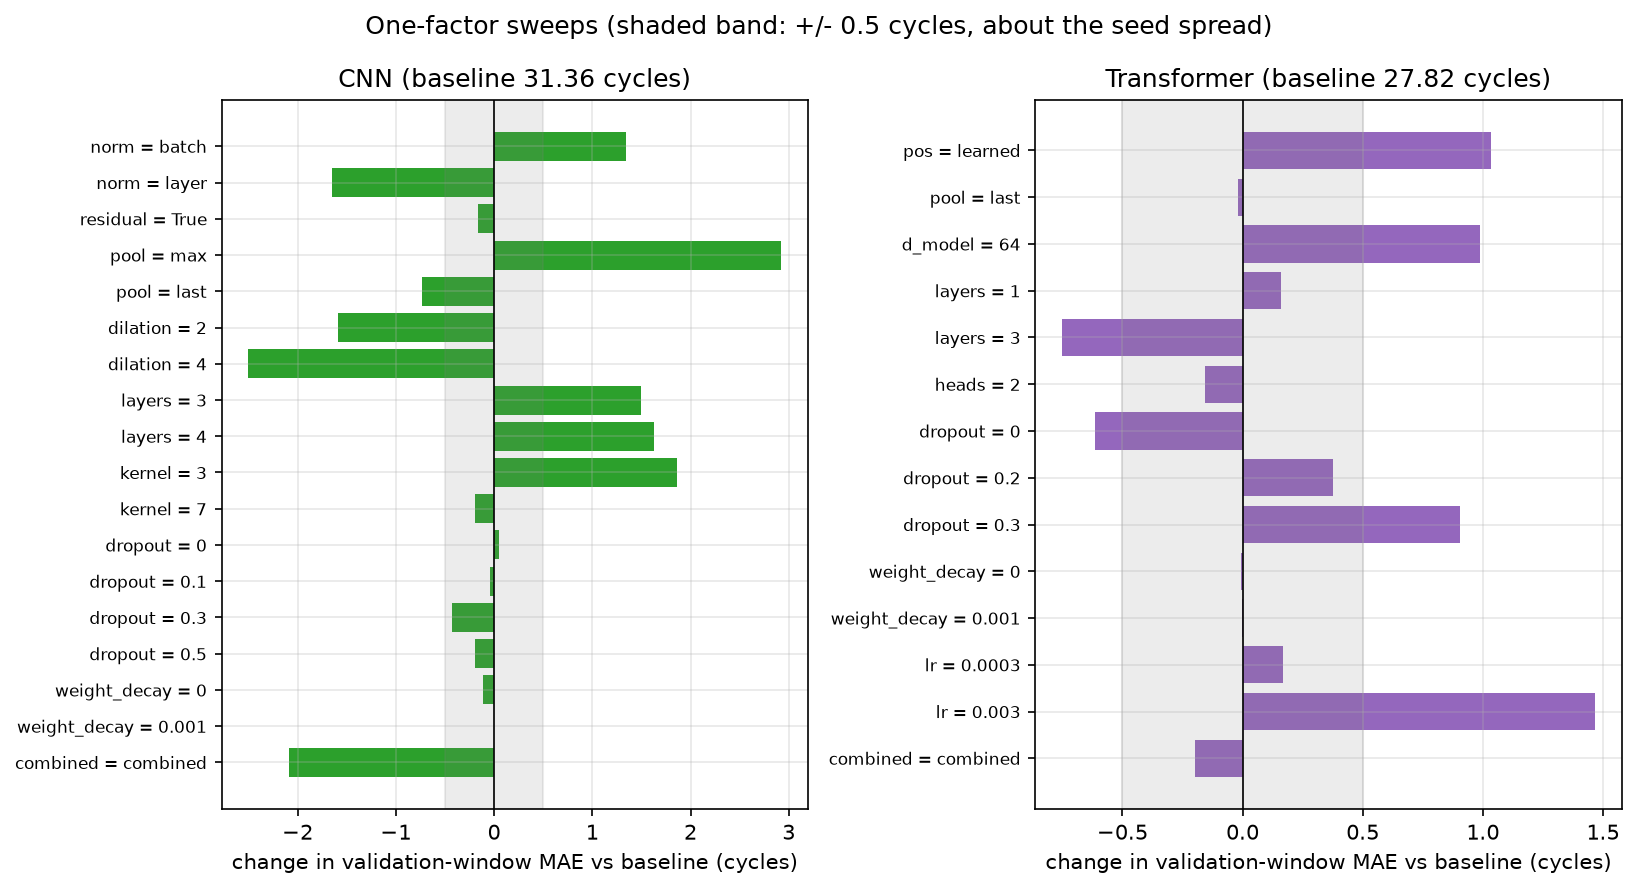
\includegraphics[width=0.85\textwidth]{../results/phase2/figures/cnn_transformer_sweeps.png}
\caption{Change in validation-engine window MAE for each one-factor change of the CNN (left) and the Transformer (right); negative values are better. The shaded band marks $\pm0.5$ cycles, about the seed-to-seed spread.}
\label{fig:cnn_sweeps}
\end{figure*}

\begin{figure}[t]
\centering
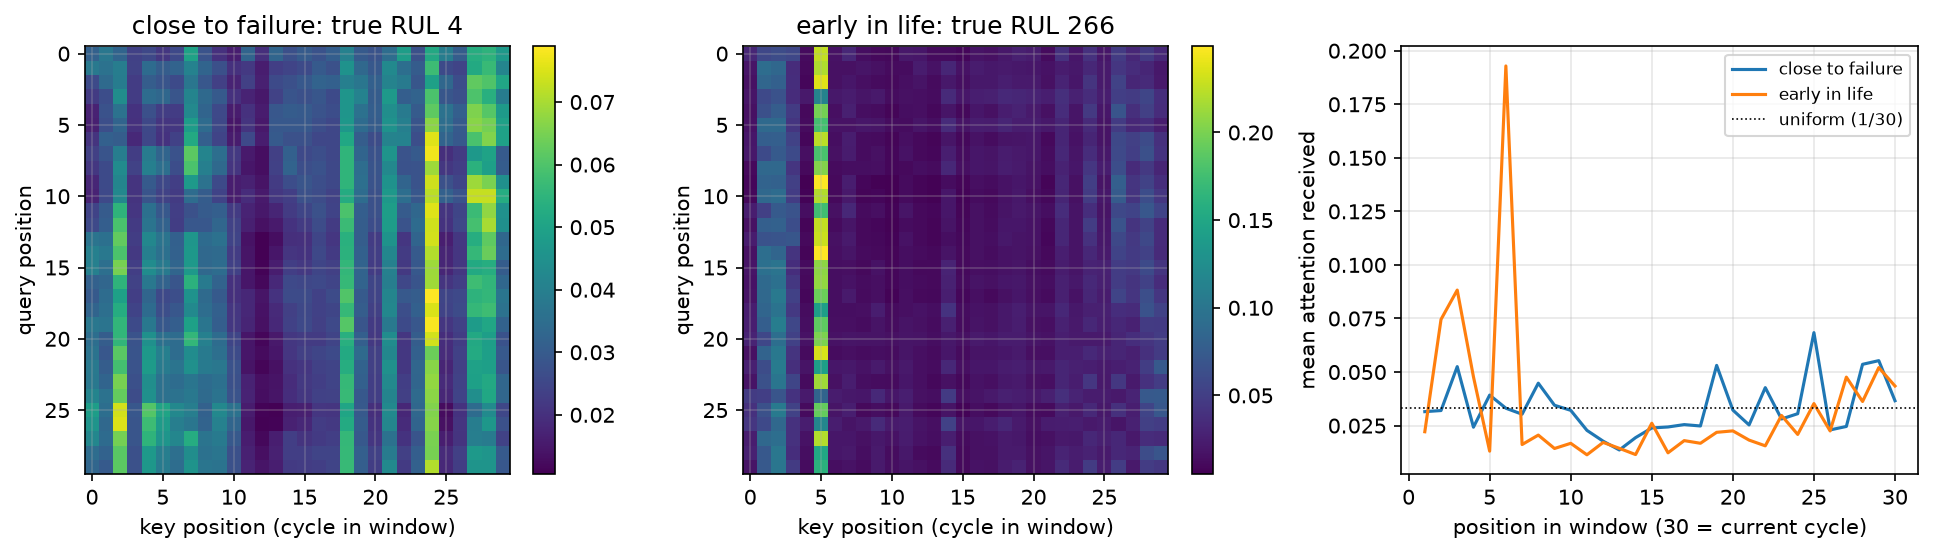
\includegraphics[width=\columnwidth]{../results/phase2/figures/transformer_attention_map.png}
\caption{First-layer self-attention (averaged over heads) of the selected Transformer for a window close to failure (true RUL 4) and one early in life (true RUL 266), and the mean attention each window position receives.}
\label{fig:attention}
\end{figure}
